% Eigenvalues of J_12(0) + 10^{-6} E_{12,1}: the 12th roots of 10^{-6}, on a circle of radius 0.316.
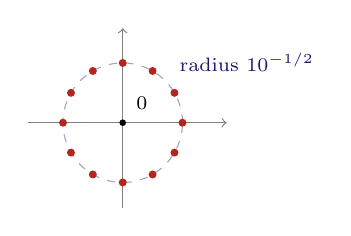
\begin{tikzpicture}[scale=2.4]
\draw[->,black!50] (-0.5,0) -- (0.55,0); \draw[->,black!50] (0,-0.45) -- (0,0.5);
\draw[MidnightBlue!40,dashed] (0,0) circle (0.3162);
\fill[BrickRed] (0.3162,0.0000) circle (0.6pt);
\fill[BrickRed] (0.2739,0.1581) circle (0.6pt);
\fill[BrickRed] (0.1581,0.2739) circle (0.6pt);
\fill[BrickRed] (0.0000,0.3162) circle (0.6pt);
\fill[BrickRed] (-0.1581,0.2739) circle (0.6pt);
\fill[BrickRed] (-0.2739,0.1581) circle (0.6pt);
\fill[BrickRed] (-0.3162,0.0000) circle (0.6pt);
\fill[BrickRed] (-0.2739,-0.1581) circle (0.6pt);
\fill[BrickRed] (-0.1581,-0.2739) circle (0.6pt);
\fill[BrickRed] (-0.0000,-0.3162) circle (0.6pt);
\fill[BrickRed] (0.1581,-0.2739) circle (0.6pt);
\fill[BrickRed] (0.2739,-0.1581) circle (0.6pt);
\fill[black] (0,0) circle (0.5pt);
\node[font=\scriptsize,anchor=south west] at (0.02,0.02) {$0$};
\node[font=\scriptsize,MidnightBlue,anchor=west] at (0.25,0.32) {radius $10^{-1/2}$};
\end{tikzpicture}
